\chapter{Implementación y experimentación}\label{chapter:implementation}
En el presente capítulo se presentan los elementos prácticos que han sido empleados para 
materializar la solución conceptualizada en el diseño previo. El objetivo principal es 
detallar cómo se implementaron las diversas tecnologías, metodologías y herramientas 
seleccionadas para construir un sistema funcional que cumpla con los 
requisitos establecidos y los objetivos trazados.

Se expondrá en primer lugar la identidad del sitio web, destacando las decisiones relacionadas 
con su diseño visual y los elementos que refuerzan su alineación con los valores de marca del 
Jardín Botánico Nacional de Cuba. Posteriormente, se describirán de manera estructurada los 
procesos técnicos y las decisiones tomadas durante la implementación, haciendo énfasis en 
aspectos clave como la selección de tecnologías, la organización del código y las estrategias 
empleadas para integrar y probar los componentes del sistema.

Además, se discutirán los retos encontrados durante esta etapa y las soluciones 
adoptadas para superarlos, asegurando que el producto final sea técnicamente robusto 
y alineado con las necesidades del proyecto.

Se explicarán por separado las soluciones propuestas para las dos problemáticas 
abordadas en el capítulo anterior. Este enfoque se adopta porque cada problemática puede 
considerarse un problema independiente, lo que facilita una comprensión más clara y detallada 
de la solución final.

Adicionalmente, se incluyen las primeras pruebas experimentales realizadas con la solución implementada, 
con el fin de evaluar su desempeño y validar que los resultados obtenidos cumplen con las 
expectativas definidas en las fases iniciales. Estos experimentos no solo verifican el cumplimiento 
funcional, sino que también permiten identificar posibles áreas de mejora o ajuste, 
garantizando que el sistema sea escalable y adaptable a futuros requerimientos.



\section{Identidad del sitio}
El sistema desarrollado como resultado de este trabajo ha sido nombrado\newline \textbf{BotaniQ}, un nombre 
que refleja de manera directa su propósito y esencia. La elección de este nombre surge de la 
combinación de dos elementos clave: la palabra \textit{``botánica''}, que alude al estudio de las plantas, 
y la letra \textit{``Q''}, que hace referencia a \textit{``query''} (significa consulta en inglés),
resaltando su función principal como una herramienta para la consulta y gestión de información sobre plantas medicinales. 
Este nombre busca transmitir simplicidad, profesionalismo y un enfoque claro en la temática del 
proyecto, a la vez que facilita su identificación y asociación con su objetivo principal.
En la Figura \ref{fig:botaniq} se muestra el logotipo de BotaniQ.

\begin{figure}[ht!]
    \centering
    
\includegraphics[width=0.25\textwidth]{Images/botaniq.png}
    \caption{Logotipo de BotaniQ}
    \label{fig:botaniq}
\end{figure}

Las interfaces de BotaniQ están diseñadas para reflejar y reforzar un valor de marca que pueda 
asociarse directamente con el Jardín Botánico Nacional de Cuba. Para lograr este propósito, 
se ha adoptado una paleta cromática basada en los colores primario y secundario presentes en 
el logotipo de dicha institución, asegurando así una identidad visual coherente y representativa.
La paleta de colores se muestra en la Figura \ref{fig:palette}.

\begin{figure}[ht!]
    \centering
    
\includegraphics[width=1\textwidth]{Images/palette.png}
    \caption{Paleta de colores}
    \label{fig:palette}
\end{figure}

Para garantizar que el diseño del sitio web BotaniQ transmita una identidad visual acorde a su 
propósito, se seleccionaron fuentes tipográficas que equilibran profesionalismo, claridad y frescura, 
alineadas con la temática botánica y científica del proyecto. Estos estilos son accesibles
libre de costo desde el sitio: \href{https://fonts.google.com/}{Google Fonts}. 
Una muestra de estos estilos se puede apreciar en la Figura \ref{fig:fonts}.

\begin{itemize}
    \item Estilo primario: \texttt{Montserrat Alternates}
    \item Estilo secundario: \texttt{Quicksand}
    \item Estilo complementario: \texttt{Sniglet}
\end{itemize}


\begin{figure}[ht!]
    \centering
    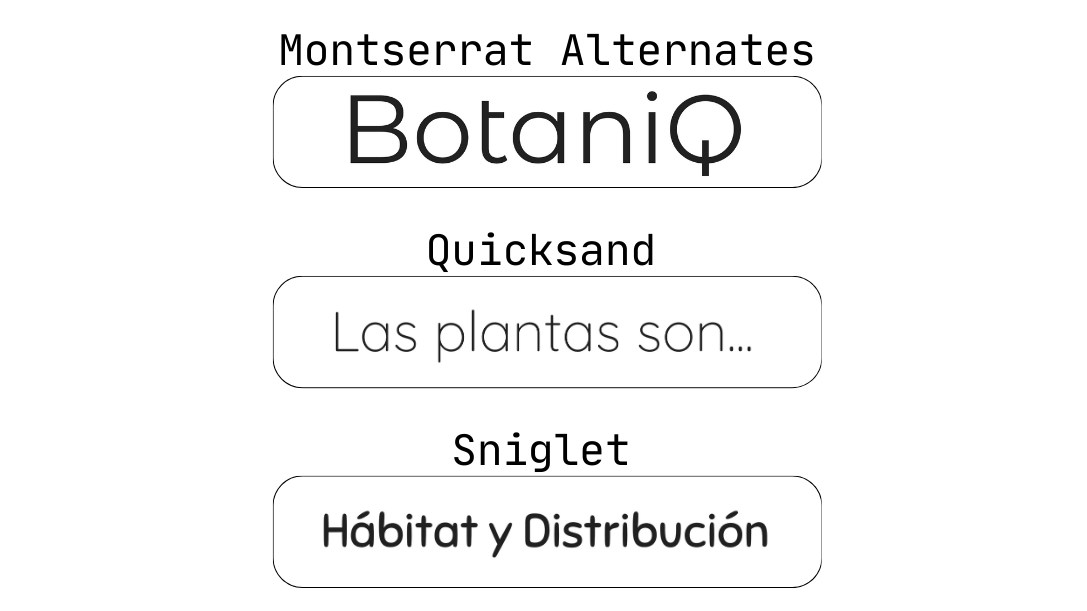
\includegraphics[width=1\textwidth]{Images/fonts.png}
    \caption{Fuentes tipográficas}
    \label{fig:fonts}
\end{figure}



\section{Solución al problema de Extracción de información}
Para implementar esta solución, se seleccionó 
\textbf{Python}\footnote{Visitar en \url{https://www.python.org}} como lenguaje de programación 
debido a su versatilidad, facilidad de uso y la sólida comunidad que lo respalda, ofreciendo 
una amplia variedad de bibliotecas para diversas tareas. Python es un lenguaje de 
programación interpretado, de alto nivel y multiparadigma, que permite trabajar con estilos 
como la programación orientada a objetos, funcional y procedimental. Su diseño enfatiza la 
legibilidad del código, lo que facilita el desarrollo y mantenimiento de proyectos.

En este contexto, se eligieron las bibliotecas 
\texttt{PyMuPDF}\footnote{Visitar en \url{https://pypi.org/project/PyMuPDF/}} y 
\texttt{pdfplumber}\footnote{Visitar en \url{https://pypi.org/project/pdfplumber/}} para 
abordar la lectura de los documentos en formato \textit{PDF}. La biblioteca \texttt{PyMuPDF} 
fue escogida principalmente por su extensa documentación y su eficacia en la extracción de 
texto de manera uniforme, lo que resulta fundamental para garantizar una base inicial 
consistente de los datos extraídos. Por otro lado, \texttt{pdfplumber} se seleccionó por las 
ventajas que ofrece en términos de manejo del diseño del documento, particularmente su 
capacidad para identificar y encuadrar bloques de texto.

La información extraída será almacenada en un archivo en formato \textit{JSON}. Este formato 
es ampliamente utilizado en la actualidad debido a su capacidad para representar datos de 
manera estructurada y su gran adaptabilidad en los sistemas computacionales modernos. 
\textit{JSON} es un formato ligero y de fácil lectura tanto para humanos como para máquinas, 
lo que lo convierte en una opción ideal para la interoperabilidad entre diferentes sistemas 
y plataformas, especialmente en aplicaciones web y servicios API.

Tal como se expuso en el capítulo anterior, se adoptará un enfoque basado en \textit{template filling} 
para estructurar la información extraída. Las plantillas se implementarán como diccionarios de Python, 
una estructura de datos que permite almacenar información en pares clave-valor de forma eficiente. 
Los diccionarios son fundamentales para garantizar una representación coherente y ordenada de los datos, 
facilitando su posterior transformación al formato \textit{JSON}.

Para la implementación del flujo de llenado de plantillas, se adoptó un estilo de programación imperativa. 
El llenado de las plantillas 
se realizó de manera jerárquica, progresando desde los niveles más generales hacia los más específicos. 
En otras palabras, primero se completaron los atributos simples de la plantilla principal, y posteriormente 
se procedió al llenado de los atributos que corresponden a subplantillas.

Este enfoque permite encapsular las reglas de llenado de las subplantillas en algoritmos independientes, 
lo que no solo mejora la modularidad del código, sino que también facilita la comprensión y el mantenimiento 
del flujo de trabajo. Al trabajar con subplantillas de manera autónoma, se asegura que cada componente de la 
plantilla sea manejado de forma eficiente y aislada, reduciendo la complejidad del sistema general y permitiendo 
futuros ajustes o ampliaciones de manera más sencilla.

Durante el desarrollo del algoritmo para la extracción de las monografías, surgieron ciertos problemas que 
requirieron ser resueltos sobre la marcha. Estas dificultades se debieron, en algunos casos, a excepciones 
en las reglas de llenado previamente definidas, ya sea por errores tipográficos en el texto original o por 
inconsistencias durante el proceso de extracción del contenido del libro. Entre los problemas identificados 
se encuentran los siguientes:

\begin{itemize}
    \item Secciones en las que no se detectó la palabra clave que determina su inicio fueron insertadas 
    erróneamente como una continuación de la sección previamente identificada.
    \item Duplicación de nombres de monografías idénticos, lo que generaba conflictos al intentar 
    utilizarlos como claves en los atributos de la plantilla.
    \item Inclusión de pies de página de las imágenes dentro del texto extraído.
    \item Inclusión de números de página entre el texto.
    \item Fragmentación de palabras en el texto debido al uso de guiones (\texttt{-}) cuando estas no 
    cabían en la línea del texto original, lo que afectaba la integridad del texto plano extraído.
\end{itemize}

La solución a estos problemas no fue particularmente compleja de identificar. Algunos casos, debido a su 
naturaleza limitada y a la falta de un patrón recurrente en el texto, fueron resueltos de forma directa 
y específica mediante soluciones personalizadas adaptadas a cada caso puntual.

Al finalizar el algoritmo de extracción, cada atributo que almacena una cadena de texto queda representado 
en un formato plano. Esto significa que no se preservan las separaciones de párrafos, siendo el contenido 
una simple secuencia de oraciones concatenadas. Además, en ocasiones donde el texto original contiene 
listas de elementos, estas se presentan como elementos continuos separados únicamente por espacios. 
Este tipo de formato puede dificultar la lectura y la interpretación del contenido, lo que hace 
necesario estructurarlo de manera más clara para mejorar su comprensión. Incluso una medida sencilla, 
como la inclusión de saltos de línea (\verb|\n|), puede contribuir significativamente a mejorar la legibilidad.

Para abordar este problema, se aprovecha el poder de los modelos de lenguaje para interpretar y 
generar texto de manera coherente. En este caso, se utilizó el modelo \texttt{gemini-1.5-flash} de
\textbf{Gemini}\footnote{Visitar a través de Google AI Studio en \url{https://aistudio.google.com/}}, desarrollado por Google, 
cuya elección se fundamenta en la disponibilidad de una API gratuita y su integración sencilla con lenguajes 
como Python para tareas automatizadas. Este modelo ha demostrado excelentes resultados en procesos de 
procesamiento y generación de texto. Para garantizar que el texto resultante cumpla con los requisitos esperados, 
se aplicaron técnicas de ingeniería de prompts diseñadas para guiar al modelo hacia la generación de resultados 
precisos y adecuados.

El resultado final es una plantilla completa, organizada y bien estructurada, con datos listos para ser leídos 
e interpretados de manera eficiente. Esta transformación mejora la presentación visual del contenido  
y optimiza su utilidad en contextos prácticos.

A continuación, se procedió a extraer la información correspondiente a la agrupación de plantas según sus aplicaciones. 
Similar al caso anterior, se presentaron algunos inconvenientes debido a inconsistencias en las reglas definidas 
durante el diseño de la solución o a limitaciones inherentes a la biblioteca utilizada para la extracción de texto. 
Entre los problemas identificados se encuentran:
 
\begin{itemize}
    \item En ciertos casos puntuales, nombres de plantas que continúan en la siguiente línea no fueron 
    detectados correctamente. Esto ocurrió porque, al no estar separados por un guion (\texttt{-}), 
    no se considera un corte de palabra, y la palabra en la línea siguiente comienza con mayúscula, 
    lo que impide la asociación automática.
    \item En un caso específico, un nombre de aplicación no fue identificado en su posición correspondiente, 
    lo que resultó en que su contenido fuera erróneamente incluido dentro de la aplicación anterior.
\end{itemize}

Dado que estos problemas son casos excepcionales y no recurrentes, se abordaron mediante correcciones 
directas en el código implementado.

El resultado final es una plantilla estructurada y completamente llena, representada en formato \textit{JSON}, 
que está lista para ser utilizada en otros entornos computacionales. 




\section{Solución al problema del Sistema de gestión y visualización: BotaniQ}
En el desarrollo de BotaniQ, se emplearon tecnologías modernas y ampliamente utilizadas en la industria 
para garantizar un sistema robusto, eficiente y escalable. Estas herramientas fueron seleccionadas 
cuidadosamente para abordar los requerimientos específicos del proyecto, permitiendo una implementación 
organizada y una experiencia de usuario óptima.

Para el frontend, se utilizó 
\textbf{React}\footnote{Visitar en \url{https://react.dev}}
en combinación con 
\textbf{TypeScript}\footnote{Visitar en \url{https://www.typescriptlang.org}}. 
React es una biblioteca de JavaScript enfocada en la creación de interfaces de usuario dinámicas y reactivas, estructuradas en componentes 
modulares que facilitan el desarrollo y la reutilización de elementos visuales. TypeScript, al ser un 
superconjunto tipado de JavaScript, aporta seguridad al proceso de desarrollo, permitiendo detectar 
errores antes de la ejecución y promoviendo un código más estructurado, lo cual es esencial en un 
proyecto de esta magnitud. Esta combinación mejora la experiencia del usuario final con una 
interfaz intuitiva, y facilita el mantenimiento y la escalabilidad del sistema.

En el backend, se optó por 
\textbf{ASP.NET Core}\footnote{Visitar en \url{https://dotnet.microsoft.com/en-us/apps/aspnet}}
como marco de desarrollo, una plataforma de código abierto diseñada para construir aplicaciones modernas 
de alto rendimiento. Este framework permite desarrollar servicios web estructurados que manejan eficientemente la lógica 
del negocio y el acceso a datos. 
La implementación del backend se organizó en capas previamente definidas: la capa de datos, la capa de acceso a datos y 
la capa de servicios, cada una desarrollada como una biblioteca dinámica (DLL) utilizando
\textbf{C\#}\footnote{Visitar en \url{https://dotnet.microsoft.com/en-us/languages/csharp}}.

La información se gestiona mediante una base de datos 
\textbf{PostgreSQL}\footnote{Visitar en \url{https://www.postgresql.org}}, 
un sistema de gestión de bases de datos relacional reconocido por su rendimiento y capacidad para manejar datos estructurados. 
El backend es responsable de procesar las solicitudes, interactuar con PostgreSQL a través de la capa de acceso a datos y exponer 
los datos mediante servicios web que pueden ser consumidos por el frontend.

Estas tecnologías trabajan de forma integrada para garantizar 
un flujo de datos coherente y confiable entre el cliente y el servidor, asegurando que los usuarios de 
BotaniQ puedan acceder a la información de manera rápida y eficiente. Estas herramientas modernas y 
probadas en entornos de producción aseguran que el sistema sea robusto, mantenible y esté preparado para 
futuros requerimientos.

Esta estructura tecnológica se ilustra en la Figura \ref{fig:techs}, proporcionando una visión 
clara de cómo se integran los diferentes componentes del sistema.

\begin{figure}[ht!]
    \centering
    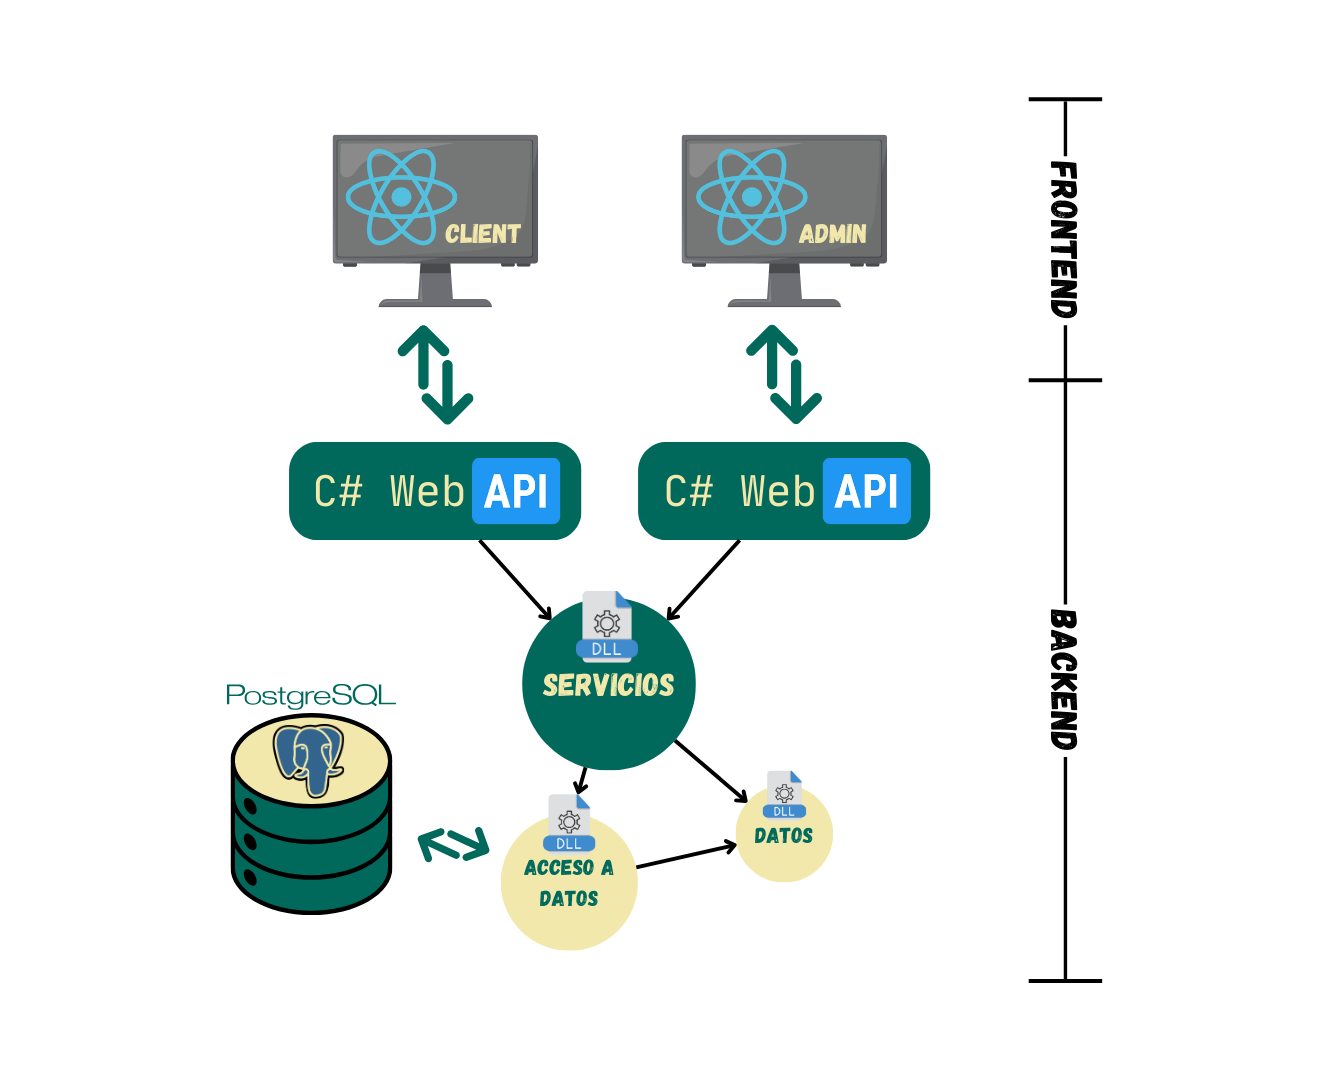
\includegraphics[width=0.9\textwidth]{Images/techs.png}
    \caption{Estructura tecnológica del sistema}
    \label{fig:techs}
\end{figure}

En ambos proyectos de frontend de BotaniQ, el desarrollo se realizó siguiendo el diseño de identidad del sitio, 
que se basa en ofrecer una experiencia visual coherente y profesional que refleje la marca asociada al 
Jardín Botánico Nacional de Cuba. A lo largo del proceso de implementación, se prestó especial atención a la 
adaptabilidad de la interfaz, asegurando que el sitio fuera completamente responsivo y brindara una experiencia 
de usuario óptima en diversos dispositivos, desde computadoras de escritorio hasta teléfonos móviles y tabletas.

Para lograr esta adaptabilidad, se utilizó 
\textbf{Tailwind CSS}\footnote{Visitar en \url{https://tailwindcss.com}},
un framework de CSS altamente flexible y eficiente que permite una personalización precisa y una creación de 
interfaces de usuario rápida y efectiva. Con Tailwind, fue posible aplicar un enfoque de diseño móvil primero, 
garantizando que la interfaz respondiera de manera eficiente a las diferentes resoluciones de pantalla sin 
perder la coherencia en su estructura visual. Además, el uso de clases utilitarias de Tailwind facilitó el 
diseño modular, lo que mejoró la mantenibilidad y escalabilidad del sistema.

Adicionalmente, se implementó 
\textbf{Flowbite}\footnote{Visitar en \url{https://flowbite.com}},
una biblioteca de componentes basada en Tailwind CSS, para acelerar el desarrollo y asegurar una interfaz de 
usuario consistente. Flowbite proporcionó una serie de componentes preconstruidos y personalizables, como 
botones, formularios y modales, lo que permitió integrar elementos interactivos con facilidad y sin necesidad 
de construir cada componente desde cero. Gracias a la combinación de Tailwind y Flowbite, se logró una 
interfaz visualmente atractiva, funcional y alineada con los principios de diseño del sitio.

Por otro lado, en el desarrollo del backend de BotaniQ, se implementaron las APIs necesarias para exponer 
los servicios que permiten la interacción entre el frontend y la base de datos. Estas APIs fueron diseñadas 
cuidadosamente para garantizar que solo se expusieran los servicios relevantes a cada uno de los dos proyectos de Web API. 
De manera específica, se desarrollaron APIs exclusivas para el módulo de administración, que permiten realizar operaciones 
de gestión sobre los datos del sistema. Esto contribuye a una arquitectura más organizada y segura, restringiendo el 
acceso a datos innecesarios y asegurando que los usuarios del módulo de administración tengan control total sobre el contenido, 
mientras que el módulo orientado al cliente final accede únicamente a los servicios de visualización.

Para la interacción con la base de datos, se utilizó 
\textbf{Entity Framework Core}\footnote{Visitar en \url{https://www.nuget.org/packages/EntityFramework}} 
como Object-Relational Mapper (ORM),
bajo un enfoque \textit{``Code First''}, lo que permitió definir las entidades de la base de datos directamente 
en el código. 
Un ORM es una herramienta que permite mapear las clases de un lenguaje de programación orientado a objetos, como C\#, 
a las tablas de una base de datos relacional, simplificando la interacción con los datos al eliminar la necesidad de 
escribir consultas SQL manualmente.
Este enfoque simplificó el proceso de creación y mantenimiento del esquema de la base de datos, 
ya que las clases de C\# fueron las que definieron la estructura de las tablas y sus relaciones. Gracias a este ORM, 
se facilitó la gestión de las entidades y la realización de consultas, permitiendo que el acceso a los datos fuera 
más eficiente y seguro.

En cuanto a la base de datos, se realizó una población inicial de la misma utilizando la información extraída del 
libro de plantas medicinales. Esta operación se ejecuta la primera vez que se inicia la Web API del administrador, 
permitiendo que los datos extraídos de manera estructurada sean cargados en la base de datos de manera automática. 
Esto asegura que la base de datos esté correctamente inicializada y preparada para su uso desde el inicio.

A pesar de utilizar PostgreSQL, un sistema de base de datos relacional con enfoque SQL, se explotaron algunas 
características que aportan la flexibilidad comúnmente asociada a las bases de datos NoSQL. PostgreSQL, 
aunque diseñado para manejar datos estructurados, ofrece funcionalidades avanzadas que permiten almacenar datos 
en formatos más flexibles, como JSON. Esta capacidad fue aprovechada para almacenar las monografías de plantas 
de manera eficiente, garantizando que, a pesar de que algunas secciones pudieran estar vacías, todas las monografías 
siguieran un esquema coherente, gracias a la técnica de \textit{template filling}. Además, se emplearon arrays 
para almacenar los vectores de los documentos, lo cual es crucial para el modelo vectorial utilizado en la búsqueda y 
comparación de textos. Estas características de PostgreSQL ofrecieron la posibilidad de trabajar con datos más 
dinámicos y flexibles, aprovechando la robustez de una base de datos relacional mientras se incorporaban elementos 
típicos de los sistemas NoSQL para facilitar una gestión más ágil y escalable de los datos.

Una característica fundamental del sistema es la capacidad de realizar búsquedas por contexto. Este mecanismo permitirá 
que el usuario pueda obtener resultados más relevantes y precisos basados en el contexto de su consulta, mejorando 
la experiencia de búsqueda y garantizando que los datos obtenidos sean los más apropiados para el usuario en cada situación. 
Este aspecto será detallado con más profundidad a continuación, pues constituye una de las funcionalidades clave incluidas en BotaniQ.


\subsection{La búsqueda por contexto}
La implementación de este mecanismo de búsqueda se lleva a cabo a través de varios componentes interconectados que incluyen controladores, 
servicios y acceso a la base de datos.

El Controlador de Consulta actúa como el punto de entrada para las solicitudes HTTP. En este caso, se encarga de gestionar las consultas de 
búsqueda que los usuarios envían a través de la API. El controlador no realiza el procesamiento de la búsqueda directamente, sino que delega 
esta tarea al servicio de búsqueda. Una vez que la consulta es recibida por el controlador, el Servicio de Búsqueda de Plantas es el responsable 
de procesarla. Este servicio contiene la lógica necesaria para analizar la consulta y calcular qué plantas de la base de datos son relevantes 
para los términos de búsqueda proporcionados.

El primer paso en el procesamiento de la consulta fue la tokenización. La entrada de texto se descompuso en unidades más pequeñas llamadas "tokens", 
que suelen ser palabras individuales o secuencias de caracteres. Durante este proceso, también se eliminaron las palabras vacías o "stop words", que 
no aportan valor semántico a la consulta. Estas palabras son descartadas para asegurar que el análisis se concentre en los términos relevantes.

Después de procesar y analizar los términos de la consulta, el siguiente paso fue buscar en la base de datos para encontrar registros 
que coincidan con estos términos. Esta búsqueda puede involucrar diferentes técnicas, tales como búsqueda 
exacta o búsqueda aproximada basada en la similitud de palabras.

En este contexto, se emplean diversos métodos, como la búsqueda exacta por término, la búsqueda basada en la distancia de Levenshtein y la búsqueda por trigramas.

La \textbf{Búsqueda Exacta por Término} fue el enfoque más sencillo y directo, en el que se busca una coincidencia exacta entre los términos de la consulta y los términos almacenados en 
la base de datos. Este tipo de búsqueda es muy eficaz cuando los términos introducidos por el usuario coinciden exactamente con los términos en la base de datos. 
Para asegurar que la búsqueda no se viera afectada por diferencias en tildes, se utilizó la función \texttt{unaccent} propia de PostgreSQL, que permite ignorar estas variaciones. 
De esta forma, las palabras ``planta'' y ``plántá'' son tratadas como equivalentes.

Sin embargo, este enfoque tiene limitaciones, ya que no es capaz de manejar errores tipográficos o variaciones menores en la escritura de los términos de búsqueda. 
En estos casos, el sistema recurre a métodos adicionales.

La \textbf{Búsqueda por Levenshtein} constituye un método adicional para ampliar la búsqueda de los posibles resultados, donde se recurre a la \textbf{distancia de Levenshtein}, que mide la cantidad mínima de ediciones necesarias 
(como inserciones, eliminaciones o sustituciones de caracteres) para convertir una cadena de texto en otra. Este método es útil cuando el usuario ha cometido errores 
tipográficos o cuando los términos de búsqueda tienen pequeñas variaciones, como en el caso de palabras mal escritas o con errores de dedo.

El algoritmo de Levenshtein calcula la ``distancia'' entre dos palabras y, en función de esa distancia, decide si la palabra almacenada en la base de datos es una 
coincidencia válida. Por ejemplo, si un usuario busca ``Abet'' y hay una palabra almacenada como ``Abey'', la distancia de Levenshtein entre estas dos palabras es 1, 
lo que indica una pequeña diferencia y hace que ``Abey'' sea un candidato adecuado.

Este tipo de búsqueda también puede implicar un umbral de distancia, donde solo las palabras cuya distancia con el término de búsqueda sea menor que un cierto valor 
(como 3) se considerarán como coincidencias válidas. Este enfoque permitió una mayor flexibilidad en la búsqueda, conviriténdolo en una solución eficiente para 
manejar errores comunes de escritura o variaciones menores.

El enfoque de \textbf{Búsqueda basada en Trigramas} es otro método potente que se utilizó para mejorar la precisión de la búsqueda, especialmente en casos donde los términos no coinciden exactamente. 
Este enfoque se basa en dividir las palabras en ``trigramas'', que son secuencias de tres caracteres consecutivos. Por ejemplo, la palabra ``planta'' se 
descompondría en los trigramas: ``pla'', ``lan'', ``ant'', ``nta''. A través de estos trigramas, el sistema puede buscar palabras que compartan secuencias similares de caracteres, 
lo que ayuda a identificar términos que son fonéticamente u ortográficamente similares al término de búsqueda.

La ventaja de utilizar trigramas es que se puede calcular la similitud entre el término de búsqueda y las palabras de la base de datos de manera rápida y eficaz. Utilizando 
técnicas como el cálculo de la \textbf{similitud de Jaccard} o el \textbf{coeficiente de similitud} de los trigramas, el sistema puede determinar qué términos en la base de datos 
son más parecidos al término buscado. Este método es especialmente útil en casos donde el usuario proporciona un término incompleto, ambiguo o incorrecto, pero cuya similitud con otros términos en la base de datos 
puede llevar a una coincidencia útil.

En PostgreSQL, este enfoque se implementa mediante la extensión \texttt{pg\_trgm}, que permite realizar búsquedas de similitud basadas en trigramas. 

En cuanto a la función de similitud utilizada en este enfoque, PostgreSQL proporciona la función \texttt{similarity}, que calcula la similitud entre dos cadenas de texto basándose en la cantidad de trigramas en común. 
Esta función es parte de la extensión \texttt{pg\_trgm} y se utiliza para comparar un término de búsqueda con los registros en la base de datos. Cuanto mayor sea el número de trigramas en común, mayor será la similitud entre las dos cadenas.

\subsubsection*{}
Una vez recuperados los documentos, el cálculo de relevancia se realizó comparando los vectores de la consulta con los de los registros devueltos como posibles resultados por la base de datos. Estos vectores se construyeron utilizando el método \textbf{TF-IDF}. Luego, con estas representaciones 
numéricas, se calculó la similitud entre ambos vectores empleando la fórmula de \textbf{similitud de coseno}. 

Finalmente, los resultados se ordenaron según su relevancia y se seleccionaron los de mayor similitud para devolverlos al usuario. Este enfoque garantiza coincidencias precisas y flexibles, adaptándose a variaciones en la entrada del usuario 
y mejorando la experiencia de búsqueda contextual.



\section{Experimentación}
intro

\subsection{Entorno de Pruebas}
Para evaluar el desempeño y la eficiencia del sistema desarrollado, se definió un entorno de pruebas controlado 
que permite obtener mediciones representativas de su funcionamiento en condiciones reales de uso. A continuación, 
se detallan los aspectos clave del entorno utilizado para la experimentación.

Las pruebas se realizaron en un equipo con las siguientes especificaciones técnicas:

\begin{itemize}
    \item \textbf{Procesador:} Intel(R) Core(TM) i7-10510U (8 CPUs ~ 2.3 GHz).
    \item \textbf{Memoria RAM:} 16 GB DDR4.
    \item \textbf{Almacenamiento:} SSD NVMe de 512 GB.
    \item \textbf{Sistema Operativo:} Windows 11 Pro.
    \item \textbf{Conexión a la base de datos:} Entorno local.
\end{itemize}

Este hardware fue seleccionado para simular un entorno de producción estándar, asegurando un rendimiento 
adecuado en la ejecución de consultas y procesamiento de datos.

El sistema fue evaluado utilizando la siguiente configuración de software:

\begin{itemize}
    \item \textbf{Backend:} ASP.NET Core 9 con Entity Framework Core.
    \item \textbf{Base de Datos:} PostgreSQL 17.2.
    \item \textbf{Cliente Web:} React 18.3.1 con Vite 4.3.3 y Tailwind CSS.
    \item \textbf{Servidor de Pruebas:} Servidor local.
    \item \textbf{APIs y comunicación:} RESTful APIs consumidas mediante llamadas HTTP con Axios.
    \item \textbf{Herramientas de monitoreo:} pgAdmin 4 para la gestión de la base de datos y Swagger para pruebas de API.
\end{itemize}

Para evaluar el funcionamiento del sistema, se empleó el conjunto de datos basado en el contenido estructurado 
de las monografías del libro \textit{``Plantas Medicinales, Aromáticas o Venenosas de Cuba''}, cargados en la población inicial, 
y que constituyen también los datos iniciales del sistema una vez en fase de producción. Se generaron y 
almacenaron los datos con las siguientes características:

\begin{itemize}
    \item \textbf{Cantidad de registros:} Las 600 monografías de plantas medicinales del libro.
    \item \textbf{Número de términos indexados:} Se identificaron ??????? términos utilizados en el modelo de espacio vectorial.
    \item \textbf{Distribución de datos:} Monografías con diferentes niveles de complejidad y extensión para evaluar las búsquedas.
\end{itemize}





\subsection{Experimentos Realizados}
Para evaluar la efectividad del sistema desarrollado, se llevaron a cabo una serie de experimentos centrados en la presentación 
de información, la eficiencia del sistema de búsqueda y el funcionamiento del módulo administrativo. Estos experimentos permitieron 
verificar que el sistema cumple con los requerimientos del sistema y detectar posibles mejoras en su implementación.

\subsubsection*{Experimento 1: Evaluación de la Presentación de Información}
\paragraph{Objetivo:}
Verificar que las monografías de plantas medicinales y las secciones adicionales del libro se presentan de manera estructurada, 
clara y accesible para los usuarios.
\paragraph{Metodología:}
\begin{itemize}
    \item Se realizaron pruebas de usabilidad con un grupo de usuarios, incluyendo relacionados con la botánica y público general.
    \item Se evaluó la facilidad de navegación en las monografías, asegurando que las secciones como nombres científicos, hábitat, 
    propiedades medicinales y composición química fueran comprensibles y organizadas.
    \item Se midió el tiempo promedio que tardaban los usuarios en encontrar información específica dentro de una monografía.
    \item Se verificó que la presentación de secciones adicionales del libro (agrupación de plantas por aplicaciones) fuera 
    accesible y fácil de entender.
    \item Se solicitó retroalimentación sobre la claridad de la interfaz y la disposición de los datos.
\end{itemize}
\paragraph{Resultados Esperados:}
\begin{itemize}
    \item Presentación estructurada de las monografías y las secciones adicionales, con un diseño intuitivo.
    \item Accesibilidad rápida a la información sin confusión ni ambigüedades.
    \item Identificación de mejoras en la interfaz para optimizar la experiencia del usuario.
\end{itemize}

\vspace{2cm}
\subsubsection*{Experimento 2: Evaluación del Mecanismo de Búsqueda}
\paragraph{Objetivo:}
Determinar la efectividad del sistema de búsqueda al recuperar información relevante tanto por nombre de planta 
como por contexto dentro de su monografía.
\paragraph{Metodología:}
\begin{itemize}
    \item Se diseñaron consultas de prueba con términos clave, nombres científicos y propiedades medicinales.
    \item Se midió el tiempo de respuesta en distintos escenarios: búsqueda exacta (nombre de la planta) y búsqueda contextual (palabras clave en la monografía).
    \item Se utilizó el modelo de espacio vectorial con similitud coseno para evaluar la relevancia de los resultados en búsquedas semánticas.
\end{itemize}
\paragraph{Resultados Esperados:}
\begin{itemize}
    \item Respuestas rápidas y precisas en búsquedas exactas.
    \item Resultados relevantes en búsquedas contextuales, incluso cuando los términos no coincidan exactamente con los almacenados.
    \item Identificación de posibles ajustes en el modelo de búsqueda para mejorar la relevancia.
\end{itemize}

\vspace{2cm}
\subsubsection*{Experimento 3: Evaluación del Módulo Administrativo}
\paragraph{Objetivo:}
Verificar que el módulo administrativo permita gestionar eficientemente la información almacenada, incluyendo las monografías de plantas y las secciones adicionales del libro.
\paragraph{Metodología:}
\begin{itemize}
    \item Se probó la creación de nuevas monografías y su correcta inserción en la base de datos.
    \item Se evaluó la funcionalidad de edición y actualización de datos existentes, midiendo el tiempo de ejecución y validando la coherencia de los cambios.
    \item Se realizaron pruebas de eliminación de registros, asegurando que los datos eliminados no afectaran otras consultas ni quedaran en caché.
    \item Se verificó la gestión de las secciones adicionales del libro, permitiendo su edición y actualización por parte del administrador.
    \item Se probó el sistema de autenticación, validando que solo usuarios autorizados accedan al módulo de administración.
\end{itemize}
\paragraph{Resultados Esperados:}
\begin{itemize}
    \item Correcto almacenamiento y visualización de nuevas monografías y secciones adicionales.
    \item Modificaciones reflejadas en tiempo real sin afectar la estructura de la base de datos.
    \item Eliminación de registros sin inconsistencias ni pérdida de integridad.
    \item Acceso restringido al módulo administrativo mediante autenticación segura.
\end{itemize}



\subsection{Análisis de Resultados}
Tras la ejecución de los experimentos, se recopilaron datos que permitieron evaluar el rendimiento y la eficacia del sistema en cuanto 
a la presentación de la información, el mecanismo de búsqueda y el módulo administrativo. A continuación, se detallan los resultados 
obtenidos en cada caso.

\subsubsection*{Resultados de Experimento 1}
Las pruebas de usabilidad demostraron que la estructura y organización de las monografías facilitaron la consulta de información. 
Se identificaron los siguientes hallazgos:
\begin{itemize}
    \item \textbf{Claridad en la presentación:} La mayoría de los usuarios encontraron la interfaz intuitiva y comprendieron rápidamente 
    la disposición de las secciones dentro de cada monografía.
    \item \textbf{Tiempo de acceso a la información:} En promedio, los usuarios tardaron menos de 5 segundos en localizar una sección específica 
    dentro de una monografía, lo que indica un diseño eficiente.
    \item \textbf{Visualización de secciones adicionales:} Los usuarios pudieron acceder sin dificultades a la sección donde se agrupan las
    plantas medicinales por aplicaciones.
    \item \textbf{Retroalimentación sobre la interfaz:} Se recibieron sugerencias para mejorar la organización de ciertos elementos visuales, 
    lo que llevó a pequeños ajustes en el diseño.
\end{itemize}
En general, los resultados muestran que la representación estructurada de la información cumple con los requerimientos del sistema, 
garantizando una navegación clara y accesible.

\subsubsection*{Resultados de Experimento 2}
Las pruebas realizadas sobre el sistema de búsqueda mostraron un desempeño sólido en la recuperación de información, con resultados 
satisfactorios en diferentes escenarios:
\begin{itemize}
    \item \textbf{Búsqueda exacta:} En el 100\% de los casos, el sistema devolvió resultados correctos al buscar por nombre científico 
    o nombre vulgar de una planta.
    \item \textbf{Búsqueda contextual:} Se logró recuperar información relevante en la mayoría de los casos, incluso cuando los términos
    de búsqueda no coincidían exactamente con los almacenados.
    \item \textbf{Ranking mejorable:} El orden brindado por la función de ranking no ofrecía los mejores resultados en cuanto a relevancia
    de los documentos rescuperados en la búsqueda.
    \item \textbf{Tiempo de respuesta:} El tiempo promedio de búsqueda fue de 2 segundos, demostrando eficiencia en la recuperación de datos.
    \item \textbf{Retroalimentación:} Algunos usuarios recomendaron la implementación de sugerencias de búsqueda para minimizar los errores 
    tipográficos. Además sugieren mostrar más resultados de búsqueda en algunas ocaciones.
\end{itemize}
De forma general, el sistema de búsqueda proporciona resultados relevantes en tiempos adecuados, permitiendo consultas tanto exactas 
como contextuales con un alto grado de precisión.

\subsubsection*{Resultados de Experimento 3}
Las pruebas en el módulo administrativo confirmaron su funcionalidad y facilidad de uso para la gestión de monografías y secciones adicionales. 
Se obtuvieron los siguientes resultados:
\begin{itemize}
    \item \textbf{Creación de monografías:} Se logró insertar nuevas monografías sin errores, reflejándose correctamente en la base de datos 
    y en la interfaz de usuario.
    \item \textbf{Edición y actualización:} Los cambios realizados en los registros se aplicaron sin inconsistencias.
    \item \textbf{Eliminación de registros:} Se verificó que la eliminación de monografías y secciones adicionales no afectara otras partes 
    del sistema, asegurando integridad en la base de datos.
    \item \textbf{Demoras de actualización:} Una vez se insertan, editan o eliminan monografías, el sistema inicia un recómputo de los 
    vectores que representan a los documentos para la recuperación de información, lo que resulta en un detenimiento temporal del funcionamiento
    del sistema. Este comportamiento es inaceptable en un entorno de producción.
    \item \textbf{Gestión de secciones adicionales:} Se confirmó que los administradores podían editar y actualizar la sección donde se agrupan
    las plantas por sus aplicaciones.
    \item \textbf{Acceso restringido:} Solo los usuarios autenticados pudieron acceder al módulo administrativo, garantizando seguridad en la 
    gestión de la información.
    \item \textbf{Retroalimentación:} Algunos usuarios reportan cierta latencia en la carga del apartado de edición de plantas agrupadas por
    aplicación. Esto se debe a la carga de cantidades excesivas de información, cuando se muestra el botón de selección de planta.
\end{itemize}
En general, el módulo administrativo cumple con los requerimientos del sistema, permitiendo la gestión de las monografías y las secciones adicionales, 
con acceso restringido para mantener la integridad de los datos; aunque con la necesidad aún de optimizar el tiempo de respuesta del sistema tras
realizar operaciones sobre las monografías.
